
%%%%%%%%%%%%%%%%%%%%%%%%%%%%%%%%%%%%%%%%%%%%%%%%%%%%%%%%%%%%%%%%%%%%%%%
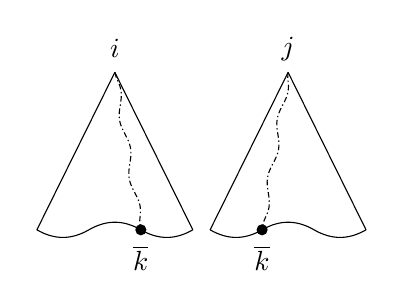
\begin{tikzpicture}[
edge from parent path=,
level distance=2cm,
level/.style={sibling distance=0.66cm/#1}
%,scale=1, every node/.style={transform shape}
]

  \tikzstyle{ref}=[circle,fill=black,inner sep=0.5mm]
  \tikzstyle{dashdot}=[dashed,dash pattern=on 2pt off 1pt on 0.5pt off 1pt]
  \tikzstyle{mysnake}=[decorate,decoration={snake,amplitude=0.4mm,segment length=0.75cm}]

  \node (c11) {}
    child { node (c12) {} }
    child { node (c13) {} }
    child { node (c14) [ref,label={below:$\overline{k}$}] {} }
    child { node (c15) {} };

  \node (c10) [minimum height=0.5cm,node distance=0.3cm,above of=c11] {$i$};

  \draw [join=round] (c11.center)
     to (c12.center) 
     to [bend right] (c13.center)
     to [bend left] (c14.center)
     to [bend right] (c15.center)
     -- cycle;

  \draw [mysnake,dashdot] (c11.center) -- (c14.center);

  \node (c21) [node distance=2.2cm,right of=c11] {}
    child { node (c22) {} }
    child { node (c23) [ref,label={below:$\overline{k}$}] {} }
    child { node (c24) {} }
    child { node (c25) {} };

  \node (c20) [minimum height=0.5cm,node distance=0.3cm,above of=c21] {$j$};

  \draw [join=round] (c21.center)
    to (c22.center) 
    to [bend right] (c23.center)
    to [bend left] (c24.center)
    to [bend right] (c25.center)
    -- cycle;

  \draw [mysnake,dashdot] (c21.center) -- (c23.center);

%  \node (c31) [node distance=2.2cm,right of=c21] {}
%    child { node (c32) {} }
%    child { node (c33) {} }
%    child { node (c34) {} }
%    child { node (c35) {} };

%  \node (c30) [minimum height=0.5cm,node distance=0.3cm,above of=c31] {$k$};

%  \draw [join=round] (c31.center)
%    to (c32.center) 
%    to [bend right] (c33.center)
%    to [bend left] (c34.center)
%    to [bend right] (c35.center)
%    -- cycle;

\end{tikzpicture}
